\documentclass[aspectratio=169,10pt]{beamer}

% ------------------------------------------------------------
% Presentation: Weather-aware itinerary project direction
% Expanded 15-20 slide version
% Author: Yit Xiaang Ztang
% ------------------------------------------------------------

\usepackage[T1]{fontenc}
\usepackage[utf8]{inputenc}
\usepackage{lmodern}
\usepackage{tikz}
\usepackage{booktabs}
\usepackage{array}
\usepackage{xcolor}
\usepackage{ragged2e}
\usetikzlibrary{arrows.meta,positioning,calc,fit,shapes.geometric}

\definecolor{DeepNavy}{HTML}{102A43}
\definecolor{MutedBlue}{HTML}{2F80ED}
\definecolor{WarmRed}{HTML}{C2410C}
\definecolor{SoftGreen}{HTML}{2F855A}
\definecolor{Purple}{HTML}{6D28D9}
\definecolor{SoftGray}{HTML}{F4F6F8}
\definecolor{DarkGray}{HTML}{475569}
\definecolor{LightBlue}{HTML}{EAF3FF}
\definecolor{LightRed}{HTML}{FFF1E8}
\definecolor{LightGreen}{HTML}{EAF7F0}
\definecolor{LightPurple}{HTML}{F3E8FF}

\setbeamertemplate{navigation symbols}{}
\setbeamertemplate{footline}{%
  \hfill\insertframenumber/\inserttotalframenumber\hspace{1em}\vspace{0.7em}}
\setbeamercolor{title}{fg=DeepNavy}
\setbeamercolor{frametitle}{fg=DeepNavy}
\setbeamerfont{title}{series=\bfseries,size=\LARGE}
\setbeamerfont{frametitle}{series=\bfseries,size=\large}
\setbeamerfont{normal text}{size=\small}
\setlength{\parskip}{0.2em}

\newcommand{\key}[1]{\textcolor{MutedBlue}{\textbf{#1}}}
\newcommand{\warn}[1]{\textcolor{WarmRed}{\textbf{#1}}}
\newcommand{\good}[1]{\textcolor{SoftGreen}{\textbf{#1}}}
\newcommand{\purple}[1]{\textcolor{Purple}{\textbf{#1}}}
\newcommand{\paper}[1]{\textcolor{DarkGray}{\footnotesize #1}}
\newcommand{\smallcite}[1]{\vspace{0.15em}{\footnotesize\textcolor{DarkGray}{#1}}}

\tikzset{
  box/.style={rounded corners=3pt, draw=DeepNavy!25, fill=SoftGray, line width=0.6pt, align=center, inner sep=5pt, minimum height=0.74cm},
  bluebox/.style={rounded corners=3pt, draw=MutedBlue!35, fill=LightBlue, line width=0.6pt, align=center, inner sep=5pt, minimum height=0.74cm},
  redbox/.style={rounded corners=3pt, draw=WarmRed!35, fill=LightRed, line width=0.6pt, align=center, inner sep=5pt, minimum height=0.74cm},
  greenbox/.style={rounded corners=3pt, draw=SoftGreen!35, fill=LightGreen, line width=0.6pt, align=center, inner sep=5pt, minimum height=0.74cm},
  purplebox/.style={rounded corners=3pt, draw=Purple!35, fill=LightPurple, line width=0.6pt, align=center, inner sep=5pt, minimum height=0.74cm},
  arrow/.style={-{Latex[length=2.1mm]}, line width=0.7pt, draw=DarkGray}
}

\title{Weather-Aware Itinerary Planning:\\From Solver-Backed Routes to Inspectable Decision Support}
\subtitle{Literature review progress, validation boundaries, and TRB vs. IUI/CHI positioning}
\author{Yit Xiaang Ztang}
\date{Meeting with Prof. Choi}

\begin{document}

% Slide 1
\begin{frame}
  \titlepage
  \vspace{-0.4em}
  \begin{center}
  \small Core framing: \key{feasible itinerary generation} + \key{human-understandable tradeoff revision}
  \end{center}
  % Speaker note: Start by saying the literature review changed the project framing. The system should not be sold as only a Gurobi travel planner.
\end{frame}

% Slide 2
\begin{frame}{Talk roadmap}
\begin{columns}[T,onlytextwidth]
\column{0.48\textwidth}
\begin{block}{What I reviewed}
\begin{itemize}
  \item Tourist Trip Design / Orienteering
  \item Personalized and context-aware itinerary recommendation
  \item LLM travel planning, symbolic validation, and LLM-as-parser systems
  \item Disruption-aware replanning
  \item HCI, explainability, mixed initiative, and plan evaluation
\end{itemize}
\end{block}

\column{0.48\textwidth}
\begin{block}{What I need feedback on}
\begin{itemize}
  \item First paper framing: TRB vs. IUI/CHI
  \item Which RQ should be central
  \item Whether language/agent functions should stay future work
  \item What empirical evidence is realistic
\end{itemize}
\end{block}
\end{columns}

\vspace{0.6em}
\centering
\colorbox{LightBlue}{\parbox{0.88\textwidth}{\centering\small The goal of this presentation is to narrow a broad prototype into a publishable research story.}}
\end{frame}

% Slide 3
\begin{frame}{Main takeaway: the contribution should shift}
\begin{columns}[T,onlytextwidth]
\column{0.49\textwidth}
\begin{block}{Weak framing}
\centering
\vspace{0.25em}
\Large ``Weather + Gurobi itinerary optimizer''
\vspace{0.25em}
\end{block}
\begin{itemize}
  \item Too close to existing TTDP / routing work
  \item Hard to claim algorithmic novelty
  \item Does not fully use the dashboard contribution
\end{itemize}

\column{0.49\textwidth}
\begin{block}{Stronger framing}
\centering
\vspace{0.25em}
\Large \textbf{Inspectable, solver-backed decision support}
\vspace{0.25em}
\end{block}
\begin{itemize}
  \item Feasible route alternatives
  \item Weather / disruption adaptation
  \item Explanations and user revision
  \item Provenance, uncertainty, and solver status
\end{itemize}
\end{columns}

\vspace{0.6em}
\centering
\colorbox{LightGreen}{\parbox{0.86\textwidth}{\centering\small The publishable gap is not only computing a plan, but helping users \textbf{understand, compare, and revise} the plan.}}
\end{frame}

% Slide 4
\begin{frame}{Progressive literature ladder: how the project angle emerged}
\centering
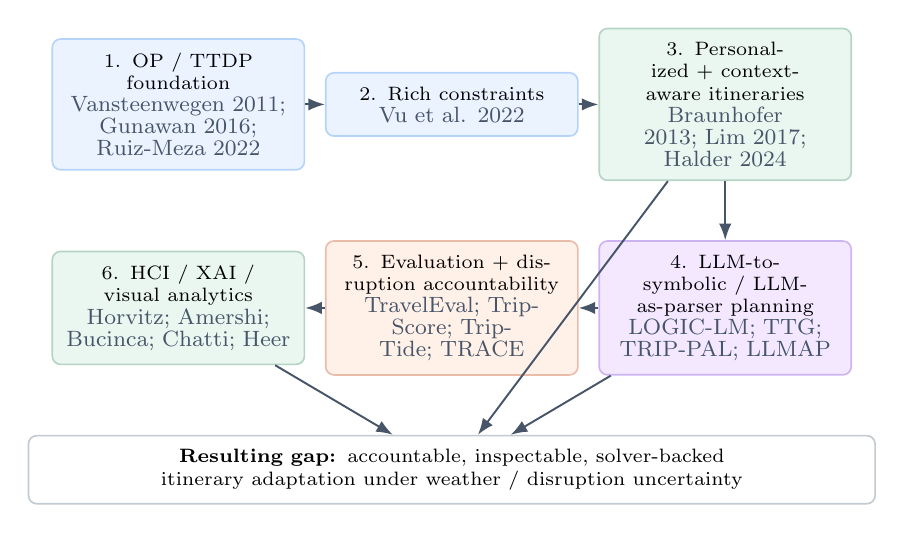
\begin{tikzpicture}[node distance=0.28cm, every node/.style={font=\scriptsize}]
\node[bluebox, text width=2.85cm] (a) {1. OP / TTDP foundation\\\paper{Vansteenwegen 2011; Gunawan 2016; Ruiz-Meza 2022}};
\node[bluebox, text width=2.85cm, right=0.25cm of a] (b) {2. Rich constraints\\\paper{Vu et al. 2022}};
\node[greenbox, text width=2.85cm, right=0.25cm of b] (c) {3. Personalized + context-aware itineraries\\\paper{Braunhofer 2013; Lim 2017; Halder 2024}};
\node[purplebox, text width=2.85cm, below=0.75cm of c] (d) {4. LLM-to-symbolic / LLM-as-parser planning\\\paper{LOGIC-LM; TTG; TRIP-PAL; LLMAP}};
\node[redbox, text width=2.85cm, left=0.25cm of d] (e) {5. Evaluation + disruption accountability\\\paper{TravelEval; TripScore; TripTide; TRACE}};
\node[greenbox, text width=2.85cm, left=0.25cm of e] (f) {6. HCI / XAI / visual analytics\\\paper{Horvitz; Amershi; Bucinca; Chatti; Heer}};

\draw[arrow] (a) -- (b);
\draw[arrow] (b) -- (c);
\draw[arrow] (c) -- (d);
\draw[arrow] (d) -- (e);
\draw[arrow] (e) -- (f);

\node[box, fill=white, text width=10.4cm, below=0.75cm of e] (gap) {\textbf{Resulting gap:} accountable, inspectable, solver-backed itinerary adaptation under weather / disruption uncertainty};
\draw[arrow] (f) -- (gap);
\draw[arrow] (d) -- (gap);
\draw[arrow] (c) -- (gap);
\end{tikzpicture}

\vspace{0.45em}
\footnotesize Recent arXiv/demo papers are useful for framing, but final publication status and scope limits must be verified before citation.
\end{frame}

% Slide 5
\begin{frame}{Literature block 1: TTDP says this is not a ranked-list task}
\begin{columns}[T,onlytextwidth]
\column{0.48\textwidth}
\begin{block}{Core problem}
\begin{itemize}
  \item Select a subset of POIs
  \item Sequence them into feasible days
  \item Respect time, distance, budget, and lodging constraints
  \item Maximize collected trip value
\end{itemize}
\smallcite{Vansteenwegen et al. 2011; Gunawan et al. 2016; Ruiz-Meza and Montoya-Torres 2022}
\end{block}

\column{0.48\textwidth}
\begin{block}{Implication for my project}
\begin{itemize}
  \item Do not claim novelty for basic POI selection + routing
  \item Use Tourist Trip Design Problem (TTDP) as the formal foundation
  \item Focus novelty on weather adaptation, route alternatives, and user-facing inspection
\end{itemize}
\end{block}
\end{columns}

\vspace{0.5em}
\centering
\colorbox{LightRed}{\parbox{0.86\textwidth}{\centering\small A high-rating attraction is not necessarily good once travel time, daily budget, weather, and hotels are considered.}}
\end{frame}

% Slide 6
\begin{frame}{Literature block 2: rich constraints create hidden feasibility failures}
\begin{columns}[T,onlytextwidth]
\column{0.50\textwidth}
\begin{block}{Vu et al. 2022: Branch-and-check}
\begin{itemize}
  \item Master problem selects candidate locations
  \item Subproblem checks schedule feasibility
  \item Infeasible selections generate cuts
  \item Rich constraints include mandatory visits, categories, order rules, budgets, time windows
\end{itemize}
\end{block}

\column{0.46\textwidth}
\begin{block}{Project design lesson}
\begin{itemize}
  \item Feasibility failures should not stay hidden inside the solver
  \item The dashboard should explain \textbf{why a candidate fails}
  \item ``Why skipped'' can be generated by attempted insertion or repair checks
\end{itemize}
\end{block}
\end{columns}

\vspace{0.4em}
\centering
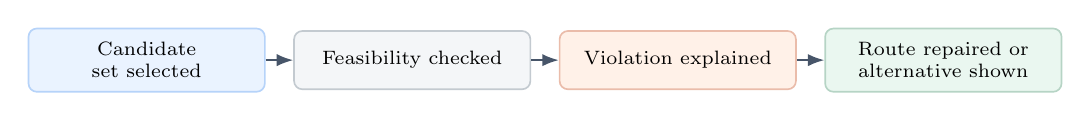
\begin{tikzpicture}[node distance=0.35cm, every node/.style={font=\scriptsize}]
\node[bluebox, text width=2.65cm] (select) {Candidate set selected};
\node[box, text width=2.65cm, right=of select] (check) {Feasibility checked};
\node[redbox, text width=2.65cm, right=of check] (reason) {Violation explained};
\node[greenbox, text width=2.65cm, right=of reason] (repair) {Route repaired or alternative shown};
\draw[arrow] (select) -- (check);
\draw[arrow] (check) -- (reason);
\draw[arrow] (reason) -- (repair);
\end{tikzpicture}
\end{frame}

% Slide 7
\begin{frame}{Literature block 3: personalization still needs feasibility}
\begin{columns}[T,onlytextwidth]
\column{0.48\textwidth}
\begin{block}{Personalized itinerary recommendation}
\begin{itemize}
  \item User interest and POI utility are necessary
  \item Context matters: time, queues, weather, crowding, seasonality
  \item But personalization alone can create infeasible routes
\end{itemize}
\smallcite{Braunhofer et al. 2013; Lim et al. 2017; Halder et al. 2024}
\end{block}

\column{0.48\textwidth}
\begin{block}{How it maps to my system}
\begin{itemize}
  \item Interest profiles and social / must-go signals estimate value
  \item Weather risk and detour cost modify realized suitability
  \item The solver decides which high-value POIs(Places of Interest) can actually fit
\end{itemize}
\end{block}
\end{columns}

\vspace{0.5em}
\centering
\colorbox{LightBlue}{\parbox{0.88\textwidth}{\centering\small The route should expose the conflict between \textbf{what the traveler likes} and \textbf{what the trip can support}.}}
\end{frame}

% Slide 8
\begin{frame}{Literature block 4: LLM planning shows why validation boundaries matter}
\begin{columns}[T,onlytextwidth]
\column{0.47\textwidth}
\begin{block}{Problem in direct LLM travel planning}
\begin{itemize}
  \item Plans can be fluent but infeasible
  \item Common failures: spatial, temporal, budget, lodging, opening-hour, and constraint violations
  \item Surface plausibility is not enough
\end{itemize}
\smallcite{TravelPlanner; TravelEval; TripScore}
\end{block}

\column{0.50\textwidth}
\begin{block}{Parser + solver direction}
\begin{itemize}
  \item Use LLMs to interpret preferences, constraints, and disruptions
  \item Compile confirmed meaning into structured planning inputs
  \item Let planner / solver verify encoded feasibility
  \item Show translation, solver/fallback, and evaluation status to users
\end{itemize}
\smallcite{LOGIC-LM; To the Globe / TTG; TRIP-PAL; LLMAP}
\end{block}
\end{columns}

\vspace{0.45em}
\centering
\colorbox{LightGreen}{\parbox{0.86\textwidth}{\centering\small This supports a language/agent future direction, but the LLM should \textbf{formulate}; it should not silently become the final route authority.}}
\end{frame}

% Slide 9
\begin{frame}{Literature block 5: TripTide gives the disruption-repair vocabulary}
\begin{columns}[T,onlytextwidth]
\column{0.32\textwidth}
\begin{block}{Disruption types}
\begin{itemize}
  \item transport
  \item accommodation
  \item restaurant
  \item attraction
  \item weather / fatigue / other
\end{itemize}
\end{block}

\column{0.32\textwidth}
\begin{block}{Severity levels}
\begin{itemize}
  \item step-level: one POI
  \item day-level: one day
  \item plan-level: whole itinerary
\end{itemize}
\end{block}

\column{0.32\textwidth}
\begin{block}{Traveler tolerance}
\begin{itemize}
  \item Flexi-Venturer: accepts rerouting
  \item Plan-Bound: wants minimal changes
  \item Evaluation: preservation of intent, responsiveness, adaptability
\end{itemize}
\end{block}
\end{columns}

\vspace{0.55em}
\centering
\colorbox{LightRed}{\parbox{0.88\textwidth}{\centering\small My project can turn weather risk into a disruption signal, then use optimization to verify repairs rather than relying on LLM-only rewriting.}}
\smallcite{TripTide 2025, treated as recent disruption-aware travel planning work}
\end{frame}

% Slide 10
\begin{frame}{Literature block 6: HCI/XAI turns routes into inspectable decisions}
\begin{columns}[T,onlytextwidth]
\column{0.50\textwidth}
\begin{block}{Design principles from HCI}
\begin{itemize}
  \item Mixed initiative: system proposes, human controls
  \item Make system capabilities and limits visible
  \item Support correction, comparison, and feedback
  \item Avoid blind overreliance on AI outputs
\end{itemize}
\smallcite{Horvitz 1999; Amershi et al. 2019; Bucinca et al. 2021}
\end{block}

\column{0.46\textwidth}
\begin{block}{Explanation design}
\begin{itemize}
  \item Why selected?
  \item Why skipped?
  \item What changed?
  \item What would need to change?
  \item What evidence / uncertainty supports this route?
\end{itemize}
\smallcite{Tintarev and Masthoff; Chatti et al. 2024; CityHood 2025; TRACE 2026}
\end{block}
\end{columns}
\end{frame}

% Slide 11
\begin{frame}{Current system: what is already useful}
\begin{columns}[T,onlytextwidth]
\column{0.48\textwidth}
\begin{block}{Implemented or partly implemented}
\begin{itemize}
  \item multi-day California route artifacts
  \item POI scoring and interest profiles
  \item hotels / base-city decisions
  \item route alternatives and trip-length alternatives
  \item weather-risk fields and map layers
  \item Gurobi-backed route components where available
  \item heuristic repair / fallback outputs
  \item source confidence and validation artifacts
  \item basic why-selected explanation text
\end{itemize}
\end{block}

\column{0.48\textwidth}
\begin{block}{Claim boundary}
\begin{itemize}
  \item Do not say every route is globally optimal
  \item Separate solver-backed from heuristic routes
  \item Browser-side interest controls may be preview-only
  \item Proxy values need uncertainty labels
  \item No user study yet proves trust or decision quality
  \item No canonical independent complete-plan evaluator yet
\end{itemize}
\end{block}
\end{columns}
\end{frame}

% Slide 12
\begin{frame}{Resulting research gap}
\begin{center}
\Large \textbf{Feasible output alone does not make a route understandable or revisable.}
\end{center}

\vspace{0.35em}
\centering
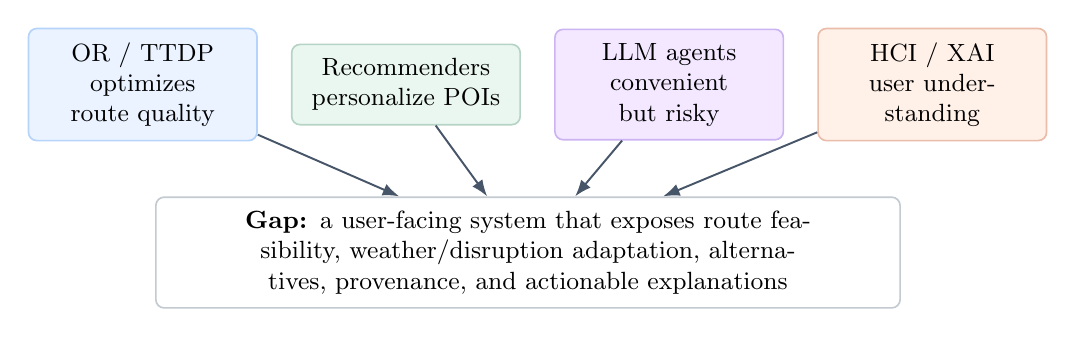
\begin{tikzpicture}[node distance=0.42cm, every node/.style={font=\small}]
\node[bluebox, text width=2.55cm] (or) {OR / TTDP\\optimizes route quality};
\node[greenbox, text width=2.55cm, right=of or] (rec) {Recommenders\\personalize POIs};
\node[purplebox, text width=2.55cm, right=of rec] (llm) {LLM agents\\convenient but risky};
\node[redbox, text width=2.55cm, right=of llm] (hci) {HCI / XAI\\user understanding};
\node[box, fill=white, text width=9.1cm, below=0.9cm of rec, xshift=1.55cm] (gap) {\textbf{Gap:} a user-facing system that exposes route feasibility, weather/disruption adaptation, alternatives, provenance, and actionable explanations};
\draw[arrow] (or) -- (gap);
\draw[arrow] (rec) -- (gap);
\draw[arrow] (llm) -- (gap);
\draw[arrow] (hci) -- (gap);
\end{tikzpicture}

\vspace{0.45em}
\centering
\colorbox{LightGreen}{\parbox{0.80\textwidth}{\centering\footnotesize Proposed contribution: \textbf{accountable, inspectable, solver-backed itinerary adaptation under frozen context}.}}
\end{frame}

% Slide 13
\begin{frame}{Proposed system framing}
\centering
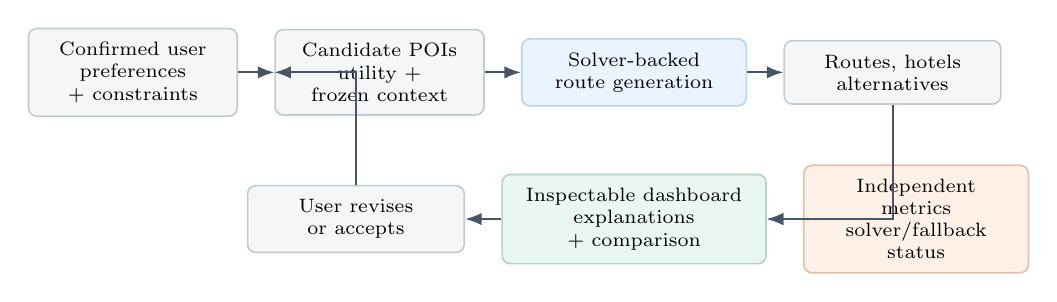
\begin{tikzpicture}[node distance=0.48cm and 0.46cm, every node/.style={font=\scriptsize}]
\node[box, text width=2.3cm] (pref) {Confirmed user\\preferences + constraints};
\node[box, text width=2.3cm, right=of pref] (poi) {Candidate POIs\\utility + frozen context};
\node[bluebox, text width=2.5cm, right=of poi] (solver) {Solver-backed\\route generation};
\node[box, text width=2.4cm, right=of solver] (alts) {Routes, hotels\\alternatives};

\node[greenbox, text width=3.0cm, below=0.85cm of solver] (dash) {Inspectable dashboard\\explanations + comparison};
\node[box, text width=2.4cm, left=of dash] (revise) {User revises\\or accepts};
\node[redbox, text width=2.5cm, right=of dash] (uncert) {Independent metrics\\solver/fallback status};

\draw[arrow] (pref) -- (poi);
\draw[arrow] (poi) -- (solver);
\draw[arrow] (solver) -- (alts);
\draw[arrow] (alts) |- (dash);
\draw[arrow] (dash) -- (revise);
\draw[arrow] (uncert) -- (dash);
\draw[arrow] (revise) |- (poi);
\end{tikzpicture}

\vspace{0.65em}
\begin{block}{Contribution statement}
\centering
A route-optimization system that turns confirmed inputs, solver output, and evaluation evidence into \textbf{inspectable evidence} for traveler decision-making.
\end{block}
\end{frame}

% Slide 14
\begin{frame}{Possible research questions}
\begin{block}{Primary RQ}
\large How can an \key{inspectable, solver-backed travel-planning interface} help users understand, compare, and revise multi-day itinerary tradeoffs under weather and disruption uncertainty?
\end{block}

\vspace{0.25em}
\begin{enumerate}
\item \textbf{Interpretation:} When preferences or disruptions are translated into planning inputs, what should require user confirmation?
\item \textbf{Explanation:} Do why-selected, why-skipped, and what-would-need-to-change explanations improve constraint understanding?
\item \textbf{Revision:} Does original-vs-adapted comparison help users make feasible revisions while preserving trip intent?
\item \textbf{Reliance:} Do provenance, uncertainty, and solver/fallback labels improve calibrated reliance rather than simply increasing trust?
\end{enumerate}
\end{frame}

% Slide 15
\begin{frame}{Agent extension: useful, but should be bounded}
\centering
\begin{center}
\resizebox{0.98\linewidth}{!}{%
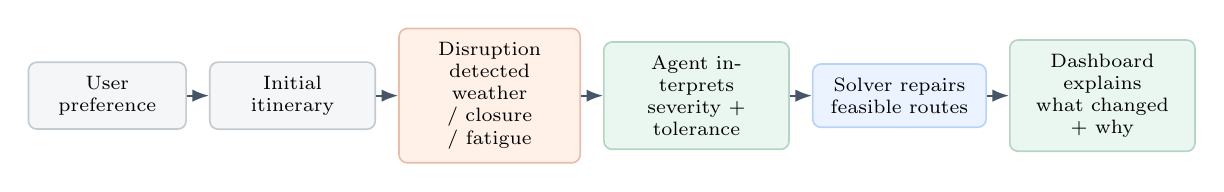
\begin{tikzpicture}[
    node distance=0.28cm,
    every node/.style={
        font=\scriptsize,
        align=center
    }
]
\node[box, text width=1.65cm] (u)
    {User\\preference};

\node[box, text width=1.75cm, right=of u] (init)
    {Initial\\itinerary};

\node[redbox, text width=1.95cm, right=of init] (dis)
    {Disruption detected\\
     weather / closure / fatigue};

\node[greenbox, text width=2.00cm, right=of dis] (agent)
    {Agent interprets\\
     severity + tolerance};

\node[bluebox, text width=1.85cm, right=of agent] (repair)
    {Solver repairs\\
     feasible routes};

\node[greenbox, text width=2.00cm, right=of repair] (explain)
    {Dashboard explains\\
     what changed + why};

\draw[arrow] (u) -- (init);
\draw[arrow] (init) -- (dis);
\draw[arrow] (dis) -- (agent);
\draw[arrow] (agent) -- (repair);
\draw[arrow] (repair) -- (explain);
\end{tikzpicture}%
}
\end{center}

\vspace{0.55em}
\begin{columns}[T,onlytextwidth]
\column{0.49\textwidth}
\begin{block}{Agent should do}
\begin{itemize}
\item parse requests into auditable fields
\item classify disruption type and severity
\item infer repair scope: stop / day / whole plan
\item translate traveler tolerance into constraints
\item compare feasible repair alternatives
\end{itemize}
\end{block}

\column{0.49\textwidth}
\begin{block}{Agent should not do}
\begin{itemize}
\item directly invent final itineraries
\item bypass feasibility checking
\item emit arbitrary solver code or hidden weights
\item silently change hotels or must-go stops
\item hide uncertainty or fallback status
\end{itemize}
\end{block}
\end{columns}
\end{frame}

% Slide 16
\begin{frame}{How to operationalize ``preservation of intent''}
\begin{columns}[T,onlytextwidth]
\column{0.45\textwidth}
\begin{block}{Optimization idea}
\small
\[
\max\; U(\text{route}) - \lambda_W R_W - \lambda_T T - \lambda_D \Delta(\text{original})
\]
\vspace{-0.5em}
\begin{itemize}
  \item utility and must-go value
  \item weather exposure penalty
  \item travel burden penalty
  \item deviation from original itinerary
\end{itemize}
\end{block}

\column{0.52\textwidth}
\begin{block}{Deviation can include}
\begin{itemize}
  \item removed or replaced POIs
  \item moved stops between days
  \item sequence changes
  \item hotel/base-city changes
  \item extra driving or cost
  \item lost semantic balance: nature, city, culture, food
\end{itemize}
\end{block}
\end{columns}

\vspace{0.45em}
\centering
\colorbox{LightBlue}{\parbox{0.86\textwidth}{\centering\small This turns ``preserve traveler intent'' from a vague goal into a measurable objective and evaluation metric.}}
\end{frame}

% Slide 17
\begin{frame}{Evaluation plan: computational + human-centered}
\begin{columns}[T,onlytextwidth]
\column{0.48\textwidth}
\begin{block}{Independent route metrics}
\begin{itemize}
  \item feasibility violations
  \item utility and selected POIs
  \item travel time, cost, and lodging changes
  \item weather exposure
  \item must-go retention
  \item preservation-of-intent score
  \item runtime, solver status, fallback status
\end{itemize}
\smallcite{TravelEval and TripScore-style complete-plan evaluation}
\end{block}

\column{0.48\textwidth}
\begin{block}{User-study metrics}
\begin{itemize}
  \item constraint-comprehension accuracy
  \item ability to explain why a stop was skipped
  \item revision quality and feasibility
  \item perceived control
  \item workload and satisfaction
  \item calibrated reliance, not just higher trust
\end{itemize}
\smallcite{HCI / XAI evaluation: Amershi, Bucinca, Knijnenburg, Chatti}
\end{block}
\end{columns}
\end{frame}

% Slide 18
\begin{frame}{Venue positioning: TRB vs. IUI or CHI}
\renewcommand{\arraystretch}{1.22}
\scriptsize
\begin{tabular}{@{}>{\raggedright\arraybackslash}p{0.16\textwidth} >{\raggedright\arraybackslash}p{0.37\textwidth} >{\raggedright\arraybackslash}p{0.37\textwidth}@{}}
\toprule
 & \textbf{TRB direction} & \textbf{IUI or CHI direction} \\
\midrule
Core angle & Transportation / operations research decision support & Intelligent interface / human-AI decision support \\
Emphasis & Route feasibility, weather disruption, robustness, travel time, lodging & Explanations, mixed initiative, user control, comparison, calibrated reliance \\
Best evidence & Computational baselines, sensitivity analysis, practical mobility implications & User study, task design, interaction logging, comprehension and revision measures \\
Best RQ & How does weather-aware solver-backed adaptation improve robust tourist mobility? & How does an inspectable interface help users understand and revise solver-backed itineraries? \\
Risk & May look less transportation-central if too interface-heavy & Needs empirical HCI evidence, not only a dashboard demo \\
\bottomrule
\end{tabular}

\vspace{0.55em}
\centering
\colorbox{LightBlue}{\parbox{0.85\textwidth}{\centering\small Current intuition: \textbf{IUI or CHI} is more distinctive if a focused user study is feasible; \textbf{TRB} is safer if the first paper emphasizes computational route adaptation.}}
\end{frame}

% Slide 19
\begin{frame}{Near-term prototype for the first study}
\begin{columns}[T,onlytextwidth]
\column{0.47\textwidth}
\begin{block}{Controlled scenario}
\begin{itemize}
\item one 7-day California itinerary
\item one explicit weather disruption
\item original route + 2--3 adapted alternatives
\item consistent evaluator for all routes
\end{itemize}
\end{block}

\begin{block}{Explanation panels}
\begin{itemize}
\item why selected
\item why skipped
\item what changed
\item what would need to change
\end{itemize}
\end{block}

\column{0.50\textwidth}
\begin{block}{Implementation cleanup}
\begin{itemize}
\item freeze scenario inputs and context snapshots
\item separate planner run, plan artifact, and evaluation report
\item compare all methods using the same metrics
\item label solver-backed vs. heuristic outputs
\item expose proxy assumptions and confidence
\item avoid post-solve route mutation without new evaluation
\item add interaction logging for study mode
\end{itemize}
\end{block}
\end{columns}
\end{frame}

% Slide 20
\begin{frame}{Possible discussion questions}
\large
\begin{enumerate}
\item Is the first contribution stronger as \key{context-aware route repair} or as an \key{inspectable decision-support interface}?
\item Which context types should be in the first paper: weather only, or weather plus closures, travel-time disruption, and pace/accessibility?
\item Is user-confirmed structured input acceptable for the first study, leaving LLM parsing as future work?
\item What baseline would be most convincing: context-blind solver, heuristic repair, full replanning, or LLM-only planning?
\item What evidence would make the paper credible for TRB versus IUI/CHI?
\end{enumerate}

\vspace{0.65em}
\centering
\colorbox{LightGreen}{\parbox{0.82\textwidth}{\centering\large Proposed near-term focus: \textbf{frozen scenario + solver-backed repair + independent evaluation + contrastive explanations}}}
\end{frame}

\end{document}
